\documentclass[twocolumn]{article}
\usepackage{graphicx}
\usepackage{amsmath}
\usepackage{hyperref}
\usepackage{xspace}
\usepackage{xparse}

\usepackage[natbib=true,backend=biber,uniquename=init,giveninits=true]{biblatex}

\addbibresource{bibl.bib}
\newcommand\erf{\ensuremath{\mathrm{erf}}\xspace}
\newcommand\erfi{\ensuremath{\mathrm{erfi}}\xspace}
\newcommand\erfc{\ensuremath{\mathrm{erfc}}\xspace}

\newcommand\dx[1]{\,\text{d}#1}

\author{Mark L. Winther}
\title{The error function}

\begin{document}
\maketitle
The error function is a mathematical special function, that occurs in probality, statistics, and partial differential equations. It got its name from J. W. L. Glasiher in 1871, who defined it while describing the "law of facility", and the chance of an error lying in an interval. The error function is defined as:
\begin{align}
\begin{split}
	\erf(x)	&= \frac{1}{\sqrt{\pi}} \int_{-x}^{x} e^{-t^2} \dx{t}\\
			&= \frac{2}{\sqrt{\pi}} \int_{0}^{x} e^{-t^2} \dx{t},
\label{eq:ferr}
\end{split}
\end{align}
and in statistics, it has the following interpetration: "for a random variable $Y$ that is normally distributed with mean 0 and variance $1/2$, $erf(x)$ describes the probability of $Y$ falling in the range $[-x,x]$."\footnote{Citation from \cite{wiki}.} A visual representation of the numerically solved error function is shown in figure \ref{fig:ferr}.

The error function's application can be rather simply interpetrated. A set of data that follows a normal distribution, that has a standard deviation $\sigma$ and expected value $0$, the probability of the error of a single measurement being between $-a$ and $a$ is described by $erf\left(\frac{a}{\sigma\sqrt{2}}\right)$.

\begin{figure}[ht]
	\centering
	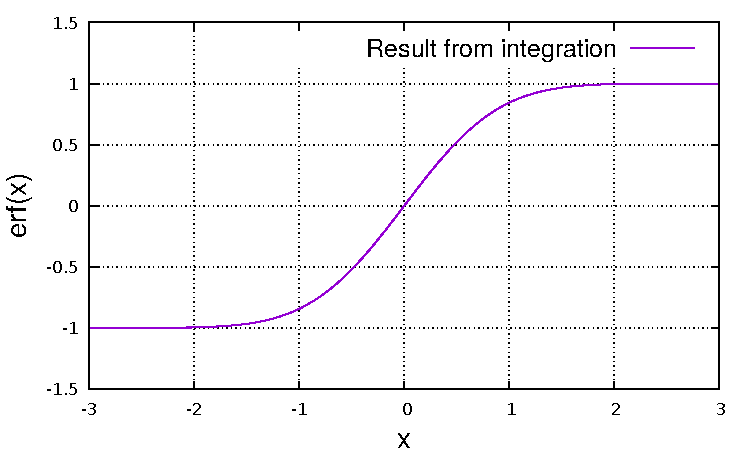
\includegraphics[width=\linewidth]{ferr.pdf}
	\caption{The error function solved numerically with a stepsize of 0.01.}
	\label{fig:ferr}
\end{figure}

There are a couple of related functions, which originates from the definition of the error function. One of them is the imaginary error function, denoted $erfi(x)$, which is defined as 
\begin{align}
\begin{split}
	\erfi (x)	&= -i \erf (ix) \\
				&= \frac{2}{\sqrt{\pi}} \int_0^x e^{t^2} \dx{t} \\
				&= \frac{2}{\sqrt{\pi}} e^{x^2} \mathrm{D}(x),
	\label{eq:iferr}
\end{split}
\end{align}
where $\mathrm{D}(x)$ is the Dawson function. Another related function is the complementary error function, denoted $\erfc(x)$, which is defined as
\begin{align}
\begin{split}
	\erfc(x)	&= 1 - \erf(x)\\
				&= \frac{2}{\sqrt{\pi}} \int_x^{\infty} e^{-t^2} \dx{t} \\
				&= e^{-x^2}\erfc\mathrm{x}(x).
	\label{eq:cferr}
\end{split}
\end{align}

This concludes the short introduction to the error function.

\printbibliography

\end{document}
